Serial Parrallel Interface (SPI) er en måde at lave hurtig seriel dataudveksling på. SPI er udviklet af Motorola og fungerer ved at man
har, som regel, en enkelt master enhed der styrer flere slave enheder. Ved SPI er der er ingen fejl-check men adressering af flere ender kan dog være 
HW krævende. I EasyWater8000 projektet er der SPI kommunikation imellem Master(devkit8000)
og Enhed(PSoC), det giver muligheden for at overføre flere data på samme tid imellem disse to.

\begin{figure}[H] \centering
{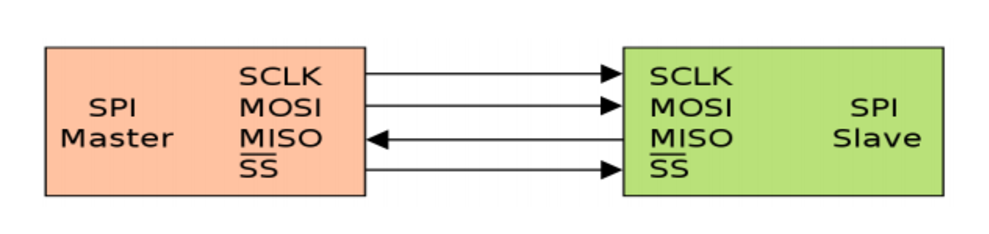
\includegraphics[width=\textwidth]{filer/design/Billeder/SPI_MASTER_SLAVE}}
\caption{SPI}
\label{lab:SPI}
\raggedright
\end{figure}

På figur \ref{lab:SPI} ses en typisk opkobling imellem Master og Slave, det kræver 4 tråde.
\begin{itemize}
 	\item SS står for "Slave select".
 	\item MISO står for "Master in slave out".
 	\item MOSI står for "Master out slave in". 
	\item SCLK står for "Serial clock" 
\end{itemize}

SPI kommunikation er baseret på skifteregister princippet, som ses på figur \ref{lab:SPI_REGISTER}. Der vælges hvilken slave der 
ønskes at skrives til ved slave select(SS), derefter shiftes et 8-bit register 1 bit ad gangen. Serial clock er den clock der sørger for at
shiftningen af bits sker korrekt, clockfrekvensen må ikke overstige grænsen for hvad enhederne kan håndtere.

\begin{figure}[H] \centering
{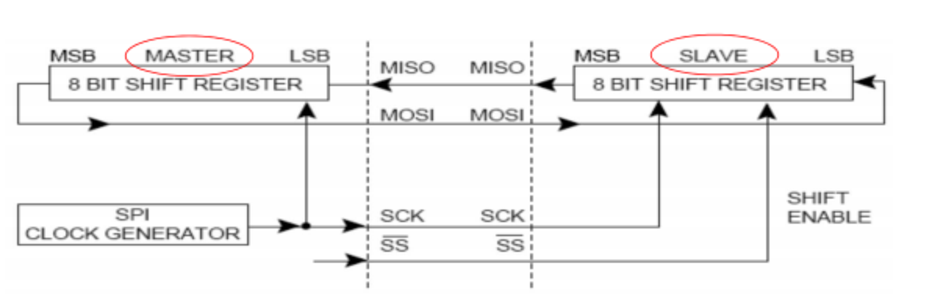
\includegraphics[width=\textwidth]{filer/design/Billeder/SPI_REGISTER}}
\caption{SPI register}
\label{lab:SPI_REGISTER}
\raggedright
\end{figure}  

En oftes anvendt kommunikation mellem master og slave foregår ved at master sætter SS til 0. Den fortæller nu til slaven at den er klar til 
dataoverførelse. Nu sender masteren en bit over til slaven og påbegynder en full duplex data transmission, samtidigt sender slaven en bit over
til masteren. Denne process fortsætter indtil masteren har sendt alle sine bits, derefter stopper masteren med at toggle på clocken og slave 
enheder bliver frigivet.

\subsection{Kernemodul og Driver}

I SPI-kommunikationen er der taget udgangspunkt i HAL Exercise 7 \footnote{Hardware abstraktioner. Exercise 7: LDD with SPI. Øvelse med SPI Kommunikation}, der er dog lavet kraftigt om i driveren, så det tilpasses EasyWater8000s behov. Kernemodulet er der ikke lavet de store ændringer i så disse beskrives ikke i projektet.

Driveren opbygges med en Skrive og en Læse metode, der begge kan læse eller skrive én 8 bits karakter(char).

\subsubsection*{Pseudokode}

\begin{lstlisting}[language=C]
int write(data){
Send data parameter ud paa SPI netvaerket
}
int read(*datapointer){
Modtag data
Flyt data til datapointer parameter
}
\end{lstlisting}

% SPI API

\subsection{SPI API}
% SPI API

SPI\_api er en klasse til at styre SPI kommunikationen. Den består af en række metoder beskrevet i afsnit \ref{fig:SPI API klassediagram}. I de følgende sektioner beskrives i pseudo-kode hvordan metoderne skal implementeres. Alle metoderne afsluttes med at sende et 'C' til Enheden. Det sørger for at TxBufferen til SPI nulstilles, så den er klar til næste opgave.

\subsubsection*{int activate(int unit) const}

Metoden skal sørge for at åbne kernefilen, skrive til den og lukke den igen.

\begin{lstlisting}[language=C]
Open file
Write 'A' to file
Write 'C' to file
Close file
Return 0
\end{lstlisting} 
\subsubsection*{int deactivate(int unit) const}

Metoden skal sørge for at åbne kernefilen, skrive til den og lukke den igen.

\begin{lstlisting}[language=C]
Open file
Write 'D' to file
Write 'C' to file
Close file
Return 0
\end{lstlisting} 
\subsubsection*{int verify(int unit) const} 

Metoden skal sørge for at åbne kernefilen, skrive til den, læse fra den og lukke den igen.
Den skal også sammenligne parameternummeret og det udlæste enhedsnummer fra Enheden og returnere 0 hvis der er et match og en fejlkode ved mismatch.

\begin{lstlisting}[language=C]
Open file
Write 'V' to file
Read unitNo from file
Parse unitNo to int
Write 'C' to file
Close file
Compare unitNo with unit
Return 0 if match
Return error if mismatch
\end{lstlisting} 
\subsubsection*{int config(int unit, float temp, float humi)} 

Metoden skal sørge for at åbne kernefilen, skrive til den og lukke den igen.
Den håndtere 2 floats, som skal konverteres til chars for at kunne sendes via SPI.

\begin{lstlisting}[language=C]
Open file
Write 'P' to file
Write temp to file
Write humi to file
Write 'C' to file
Close file
Return 0
\end{lstlisting} 
\subsubsection*{int getLog(vector<string> \&data, int * units, int size)}

Metoden sørger for at åbne kernefilen, skrive til den, læse fra den og lukke den igen.
Den udlæser et buffer array fra Enheden som pakkes ned i en vector til data parameteret.

\begin{lstlisting}[language=C]
Open file
Write 'L' to file
Read buffersize from file
Read buffer buffersize times
Build datastring if 'D' are present
Build errorstring(s) if 'E' are present
Build vector from data and errorstrings
Move vector to data
Close file
Return 0
\end{lstlisting} 


% SPI HANDLER

\subsection{SPI Handler}
% SPI Handler

SPI handleren skal være en interrupt rutine, der startes når der kommunikeres over SPI. Den skal håndtere alle metoderne fra SPI\_api. Og kalde metoder på Enhed.

\textbf{ISR}

\begin{lstlisting}[language=C]

CY_ISR()
{
switch {
    	case 'A':
		Turn on Green LED
		Call activate method:                
	case 'D':
		Turn on Red LED
		Call deactivate method:  
	case 'P':
		Turn on White LED			
		Save humidity and temperature data            
		Call config method
	case 'V':
		Turn on Purple LED  
		Write UnitNo to tx buffer  
	case 'L':
		Turn on Blue LED
		Get log data buffer
		Write data buffer to tx buffer
	case 'R':
		Write tx buffer to Master
	case 'C':
		Clear tx-buffer
		Reset spiCounter 
}
\end{lstlisting}